
\chapter{CHALLENGES}

\section{Zooko's Triangle}
\label{sec:ZookosTriangle}

Our primary objective with OnioNS is to provide human-meaningful domain names Tor hidden services, but we list distributed and securely unique domain names in our design requirements. Achieving all three objectives is not easy; a naming scheme can use a central root zone or authority to ensure that meaningful domains remain unique but then it is not distributed, it can achieve a distributed nature by generating domain names with cryptographic hash function but then domains are no longer human-meaningful, or it can allow peers to provide meaningful names to each other but then these names are not guaranteed to be globally unique. This problem is illustrated in Figure \ref{fig:ZookosTriangle} and summarized by Zooko's Triangle, a conjecture proposed by Zooko Wilcox-O'Hearn in late 2001. The conjecture states a persistent naming system can achieve at most two of these properties: it can provide unique and meaningful names but not be distributed, it can be distributed and provide unique names that are not meaningful, or it can be distributed and provide meaningful names that are not guaranteed to be unique.\cite{ferdous2009security}\cite{stiegler2005petname}

\begin{figure}[htbp]
	\centering
	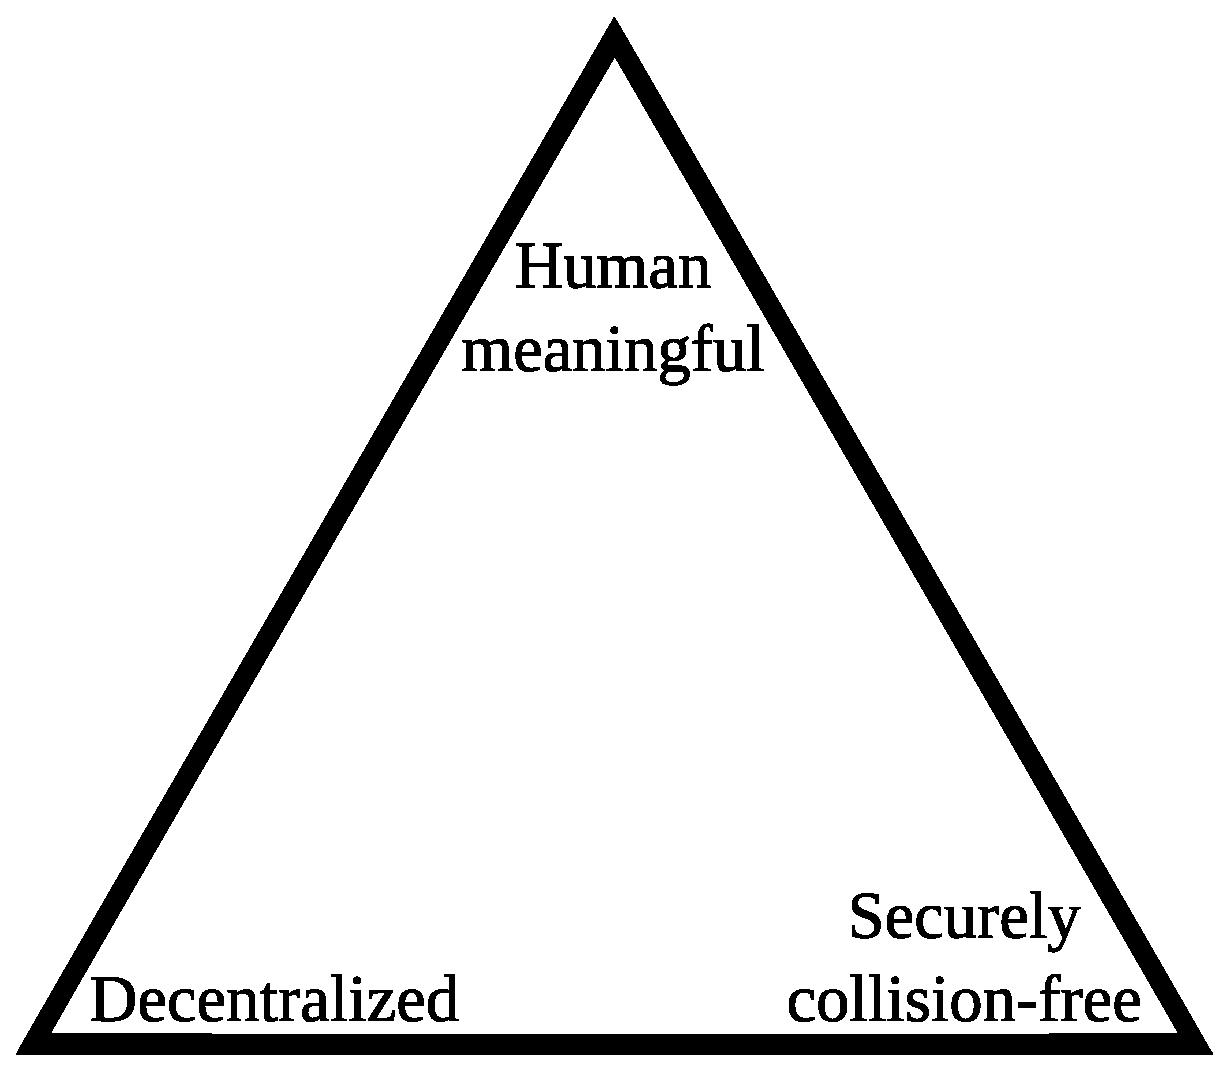
\includegraphics[width=0.3\textwidth]{images/Zooko.eps}
	\caption{Zooko's Triangle.}
	\label{fig:ZookosTriangle}
\end{figure}

Petnames are systems that achieve all three properties of Zooko's Triangle. Some examples of naming systems that achieve only two of these properties include:

\begin{itemize}
	\item \textbf{Securely unique and human-meaningful} --- Clearnet domain names are memorable and provably collision free, but they use DNS with a hierarchical structure and central authorities under the jurisdiction of ICANN.
	\item \textbf{Decentralized and human-meaningful} --- Human names and nicknames are legal and social labels for each other, but we provide no protection against name collisions.
	\item \textbf{Securely unique and decentralized} --- Tor hidden service .onion domains, PGP keys, and Bitcoin/Namecoin addresses use the large key-space and the collision-free properties of cryptographic hash algorithms to ensure uniqueness, but do not use meaningful names.
\end{itemize}

We consider the securely unique and human-meaningful properties the most important objectives, and like Namecoin (discussed in section \ref{sec:Namecoin}) we provide a mechanism that enables the network to agree on a common database and largely prevents it from fragmenting. Additionally, all participants can confirm for themselves the integrity of the database and the uniqueness of domain names contained within it. This holds the securely unique property within the distributed environment. 

\section{Non-existence Verification}

In our design requirements we specify that clients of a naming system should be able to verify the authenticity of domain names. On the Internet, this is achieved through SSL certificates: clients first receive from the destination server a digital certificate, they verify that the certificate matches the domain name they requested to their DNS resolver, and finally they check the certificate against Certificate Authorities via a Chain of Trust. Of equal importance, however, is the capability to verify the non-existence of domain names. Specifically a resolver may falsely claim that a domain name cannot be resolved because it does not exist, but a client has no mechanism by which to verify this claim besides changing resolvers. This is a weakness often overlooked in other DNSs and resolving this problem is not easy. However, we in section \ref{sec:HashtableBitset} we introduce a data structure and a protocol that allows a resolver to proof non-existence in constant time.
